%%%%%%%%%%%%%%%%%%%%%%%%%%%%%%%%%%%%%%%%%%%%%%%%%%%%%%%%%%%%%%%%%%%%%%%%%%%%%%%%
%2345678901234567890123456789012345678901234567890123456789012345678901234567890
%        1         2         3         4         5         6         7         8

\documentclass[letterpaper, 10 pt, conference]{ieeeconf}  % Comment this line out if you need a4paper

%\documentclass[a4paper, 10pt, conference]{ieeeconf}      % Use this line for a4 paper

\IEEEoverridecommandlockouts                              % This command is only needed if 
                                                          % you want to use the \thanks command

\overrideIEEEmargins                                      % Needed to meet printer requirements.

% See the \addtolength command later in the file to balance the column lengths
% on the last page of the document


% MYTHINGS
\usepackage{amssymb,amsmath, amsfonts,color}

\newtheorem{theorem}{Theorem}
\newtheorem{definition}{Definition}
\newtheorem{remark}{Remark}
\newtheorem{lemma}{Lemma}
\newtheorem{corollary}{Corollary}
\newcommand{\R}{\mathbb{R}}

% The following packages can be found on http:\\www.ctan.org
%\usepackage{graphics} % for pdf, bitmapped graphics files
%\usepackage{epsfig} % for postscript graphics files
%\usepackage{mathptmx} % assumes new font selection scheme installed
%\usepackage{times} % assumes new font selection scheme installed
%\usepackage{amsmath} % assumes amsmath package installed
%\usepackage{amssymb}  % assumes amsmath package installed
\usepackage{pdfpages}
\usepackage{siunitx} 

\title{\LARGE \bf
GP-based Model Predictive Control*
}


\author{Dimitrios Gkoutzos$^{1}$, Luzia Knödler$^{2}$ and Lucas Rath$^{3}$% <-this % stops a space
\thanks{*Project within the course Statistical Learning and Stochastic Control, University of Stuttgart, \today.}% <-this % stops a space
\thanks{$^{1}$Dimitrios Gkoutzos is a student of the Master study programm Engineering Cybernetics, University of Stuttgart,
        {\tt\small dimitrios.gk@gmx.de}}%
\thanks{$^{2}$Luzia Knödler is a student of the Master study program Engineering Cybernetics, University of Stuttgart,
        {\tt\small luzia.knoedler@web.de}}%
\thanks{$^{3}$Lucas Rath is a student of the Master study program Engineering Cybernetics, University of Stuttgart, and of the Master study program Systems, Control and Mechatronics, Chalmers University of Technology,
        {\tt\small lucasrm25@gmail.com}}%
}


\begin{document}



\maketitle
\thispagestyle{empty}
\pagestyle{empty}


%%%%%%%%%%%%%%%%%%%%%%%%%%%%%%%%%%%%%%%%%%%%%%%%%%%%%%%%%%%%%%%%%%%%%%%%%%%%%%%%
\begin{abstract}

Describe topic and relevance in a few sentences so that the reader is motivated to
read the whole paper.

\end{abstract}


%%%%%%%%%%%%%%%%%%%%%%%%%%%%%%%%%%%%%%%%%%%%%%%%%%%%%%%%%%%%%%%%%%%%%%%%%%%%%%%%
\section{INTRODUCTION}
Model predictive control (MPC) is a popular control strategy which uses a dynamic plant model to obtain the control input that optimizes future reactions of the plant~\cite{kocijan2004gaussian}. The performance of MPC depends highly on how well the model captures the dynamics of the plant~\cite{kabzan2019learning}. But the identification of such an \textit{a priori} model can be challenging and the dynamics of the plant could also change during the application~\cite{kabzan2019learning,ostafew2014learning}. Therefore, a simple and fixed nominal model of the plant can be used in combination with a learned disturbance model. The disturbance model represents the error between the observed behaviour of the plant and the behaviour of the nominal model~\cite{ostafew2014learning}. It can be modelled as a Gaussian Process (GP) regression which is a probabilistic, non-parametric model~\cite{kocijan2004gaussian}. GPs have the advantage of characterizing the prediction uncertainities~\cite{kocijan2004gaussian}. The mean estiamte of a GP can also be used to model the full dynamics of the plant and not only the model error. This approach was applied to a cart pole swing-up environment and an autonomous racing task in \cite{van2017online}. To reduce high computational costs sparce spectrum GPsare chosen. Kocijan et al.~\cite{kocijan2004gaussian} use an offline-identified GP model instead. Another alternative is the generation of local GPs (LGPs) where for each subspace of the GP input space different GPs are identified. While Nguyen-Tuong et al.~\cite{nguyen2009local} and Meier et al.~\cite{meier2014efficient} identify many LGPs, Ostafew et al.~\cite{ostafew2014learning} compute one single LGP based on data within a sliding window. Other applications of GPs in a MPC framework are .
 \\
In this report we present the results of our project within the course ``Statistical Learning and Stochastic Control''. First, our literature research on GP-based MPC is summarized. Then a short introduction to the theory of MPC and GPs is given. The implementation of two examples is presented in Section~\ref{main_results} and the results are discussed in section~\ref{examples}.\\
Starting with the Definition of the used Notation below.\\
Bold lowercase letters are used for vectors $\boldsymbol{x} \in \mathcal{R}^n$ and bold uppercase letters for matrices $\boldsymbol{X} \in \mathcal{R}^{n \times m}$. The j-th column of a matrix $\boldsymbol{X}$ is denoted by $[\boldsymbol{X}]_{.,j}$ and the element in the i-th row and j-th column is $[\boldsymbol{X}]_{ij}$. A diagonal matrix $\boldsymbol{X}$ with the diagonal elements $x_{11}, x_{22}, \cdots, x_{nn}$ is represented by $\text{diag}(x_{11}, x_{22}, \cdots, x_{nn})$. If ${w}~\sim~\mathcal{N}(\boldsymbol{\mu},\boldsymbol{\Sigma})$ $w$ is normal distributed with mean $\boldsymbol{\mu}$ and variance $\boldsymbol{\Sigma}$.

Introduce topic and describe motivation and relevance of problem/topic.

In this paper we give an introduction to the results presented in paper(s) \cite{Bro-14}.
We present the main results, discuss ideas and illustrate the results with simulations.\\

Notation. Define notation.

%%%%%%%%%%%%%%%%%%%%%%%%%%%%%%%%%%%%%%%%%%%%%%%%%%%%%%%%%%%%%%%%%%%%%%%%%%%%%%%%
\section{BACKGROUND}
In this section a revision of GPs for our application and necessary background information on MPC are presented. The revison of GPs follows Kabzan et al.~\cite{kabzan2019learning} as well as Rasmussen and Williams~\cite{williams2006gaussian}. \\

As mentioned in the Introduction, a GP is used to identify the disturbance $\boldsymbol{d_{true}}$, which describes the error between the nominal plant dynamics $f_{nom}$ and the true dynamics $f_{true}$. Thus, the true system equations are given by
\begin{align}
\begin{split}
\boldsymbol{x_{k+1}} &= f_{true}(\boldsymbol{x_k},\boldsymbol{u_k}) \\
        &=  f_{nom}(\boldsymbol{x_k},\boldsymbol{u_k}) + \boldsymbol{B_d}\big(\boldsymbol{d_{true}}(\boldsymbol{z_k})+ \boldsymbol{w}\big),
\end{split}
\end{align}
with $\boldsymbol{z_k} = \boldsymbol{B_z} \boldsymbol{x_k}$ ($\boldsymbol{B_z} \in \mathcal{R}^{n_z \times n}$) and $\boldsymbol{w}~\sim~\mathcal{N}(\boldsymbol{0},\boldsymbol{\Sigma_w})$  the gaussian measurement noise, where $\boldsymbol{\Sigma_w}= diag(\sigma_1^2, \cdots ,\sigma_{n_d}^2)$.
The disturbance $\boldsymbol{d} = \boldsymbol{d_{true}}(\boldsymbol{z_k}) + \boldsymbol{w_k}$ is identified using input and output data pairs $(\boldsymbol{z_k},\boldsymbol{y_k}=\boldsymbol{d_{true}}(\boldsymbol{z_k})+\boldsymbol{w_k})$ which are saved in a dictionary $\mathcal{D}$ of length $m$
\begin{align}
\begin{split}
\mathcal{D} = \{\boldsymbol{Z} &=[\boldsymbol{z_1}, \cdots, 		\boldsymbol{z_m}] \in \R^{n_z \times m} , \\
                \boldsymbol{Y} &=[\boldsymbol{y_{1}},\cdots,\boldsymbol{y_{m}}]\in \R^{n_d \times m} \}.
\end{split}
\end{align}
If $m>m_{max}$, the dictionary is updated by removing the oldest data pair.\\
Each output dimension $a \in \{1, \cdots, n_d\}$ is treated as a different GP with the kernel $\boldsymbol{k^a}$, which results in the posterior distribution mean $\boldsymbol{\mu^a(z)}$ and variance $\boldsymbol{\Sigma^a(z)}$
\begin{align}
\boldsymbol{\mu^a(z)} &= \boldsymbol{k_{zZ}^a}( \boldsymbol{K_{ZZ}^a} +\boldsymbol{I} \boldsymbol{\sigma_a})^{-1}[\boldsymbol{Y}]_{.,i},\\
\boldsymbol{\Sigma^a(z)} &= k_{zz}^a-\boldsymbol{k_{zZ}^a} ( \boldsymbol{K_{ZZ}^a} +\boldsymbol{I} \boldsymbol{\sigma_a})^{-1} \boldsymbol{k_{Zz}^a}
\end{align}
in dimension $a$ for a test point $\boldsymbol{z}$.
The expressions $k_{zz}^a$, $ \boldsymbol{k_{zZ}^a}$, $\boldsymbol{k_{Zz}^a}$ and $\boldsymbol{K_{ZZ}^a}$ are compact notations for $k^a(\boldsymbol{z},\boldsymbol{z}) \in \R$, $[\boldsymbol{k_{zZ}^a}]_j =k^a(\boldsymbol{z},z_j)$, $[\boldsymbol{k_{Zz}^a}]_j =k^a(z_j,\boldsymbol{z})$ and $[\boldsymbol{K_{ZZ}^a}]_{ij} = k^a(z_i,z_j)$, respectively. It holds $\boldsymbol{k_{Zz}^a}=(\boldsymbol{k_{zZ}^a})^T \in \R^m$.\\
For each output dimension $a$ we make use of the squared exponentional kernel given by
\begin{equation}
k^a(\boldsymbol{z},\boldsymbol{\bar{z}}) = \boldsymbol{\sigma_{f,a}}^2 \exp(-0.5(\boldsymbol{z}-\boldsymbol{\bar{z}})^T \boldsymbol{M}^{-1} (\boldsymbol{z}-\boldsymbol{\bar{z}})),
\end{equation}
where $\boldsymbol{\sigma_{f,a}}^2$ and $\boldsymbol{M}$ are the squared output variance and the positive diagonal length scale matrix, respectively.
The practical implementation of Gaussian process regression from page 19 of Rasmussen and Williams~\cite{williams2006gaussian} which uses the Cholesky factorization to address the matrix inversion is applied. This results in the following algorithm
\begin{align}
\boldsymbol{L^a} &= \text{cholesky}(\boldsymbol{K}(\boldsymbol{Z},\boldsymbol{Z}) + \boldsymbol{\sigma_n(a,a)}^2\boldsymbol{I})\\
\boldsymbol{\alpha^a} &= \boldsymbol{L}^T\backslash(\boldsymbol{L} \backslash \boldsymbol{Y}(:,a)),
\end{align}
where $[\boldsymbol{K}(\boldsymbol{Z},\boldsymbol{Z})]_{ij}=k(z_i,z_j)$ with $z_i, z_j \in \boldsymbol{Z}$.
Thus, the predictive mean and variance are given by
\begin{align}
\mu_y^a&=\boldsymbol{K}(\boldsymbol{z},\boldsymbol{Z})^T\boldsymbol{\alpha^a}\\
\Sigma_y^a&=k(\boldsymbol{z},\boldsymbol{z})-\boldsymbol{v^a}^T\boldsymbol{v^a},
\end{align}
with $\boldsymbol{v^a}=\boldsymbol{L^a}/\boldsymbol{K(z,Z)}$.\\
Combining the GPs of each dimension results in the multivariate GP approximation 
\begin{equation}
\boldsymbol{d}(\boldsymbol{z})\sim \mathcal{N}(\boldsymbol{\mu^d}(\boldsymbol{z}),\boldsymbol{\Sigma^d}(\boldsymbol{z})),
\end{equation}
where the mean $\boldsymbol{\mu^d(z)} \in \mathcal{R}^{n_d}$ and the variance $\boldsymbol{\Sigma^d(z)}~\in~\mathcal{R}^{n_d \times n_d}$ are given by
\begin{align}
\boldsymbol{\mu^d}(\boldsymbol{z}) &= [\mu^1(\boldsymbol{z}),\cdots, \mu^{n_d}(\boldsymbol{z})]^T,\\
\boldsymbol{\Sigma^d}(\boldsymbol{z}) &= \text{diag}([\Sigma^1(\boldsymbol{z}),\cdots, \Sigma^{n_d}(\boldsymbol{z})]).
\end{align}
The model considered for control including the identified disturbance $d$ is given by
\begin{equation}
\boldsymbol{x_{k+1}} = f_{nom}(\boldsymbol{x_k},\boldsymbol{u_k}) + \boldsymbol{B_d} \boldsymbol{d}(\boldsymbol{z_k}).
\end{equation}
 \\
Model predictive control (MPC), receding  horizon  control or moving horizon control are all names for a control strategy which predicts the future dynamic behaviour within a finite prediction horizion and chooses the control input such that a perfomance functional is minimized~\cite{allgeowernonlinear}. Since the predicted behaviour is not equal to the system behaviour due to disturbances and model-plant mismatch, only the first input of the computed control input sequence is applied~\cite{allgeowernonlinear}. Using the new measurement one sampling time later, the procedure is repeated to find a new control sequence within the receding horizon.\\
Evaluating the GP model $\boldsymbol{d}(\boldsymbol{x_k},\boldsymbol{u_k})$ results in a stochastic distribution, which leads to a stochastic distribution of the state $\boldsymbol{x}$. The distribution at each prediction step is assumed to be Gaussian with $\boldsymbol{x_k} \sim \mathcal{N}(\boldsymbol{\mu^x_k},\boldsymbol{\Sigma^x_k})$. To evaluate the uncertainity over the prediction horizon $N$ the mean and variance of $\boldsymbol{x}$ are propagated forward which results in
\begin{align}
\boldsymbol{\mu^x_{k+1}}&= f_{nom}(\boldsymbol{\mu^x_k},\boldsymbol{u_k})+\boldsymbol{B_d} \boldsymbol{\mu^d}(\boldsymbol{\mu^x_k},\boldsymbol{u_k})\\
\boldsymbol{\Sigma^x_{k+1}} &= ????.
\end{align}
For more information on the propagation see ???? Appendix.
Thus, the MPC problem is given by
\begin{align}
\min_{\tilde{u}} &\big(\sum_{k=1}^{N-1} f_o(t_k,\boldsymbol{\mu^x_k},\boldsymbol{\Sigma^x_k},\boldsymbol{\tilde{u}_k},r(t))\big) + f_{end}(t_N,\boldsymbol{\mu^x_N},\boldsymbol{\Sigma^x_N},r(t_N))\\
&\boldsymbol{\mu^x_0} = \boldsymbol{x}(t)\\
&\boldsymbol{\mu^x_{k+1}}= f_{nom}(\boldsymbol{\mu^x_k},\boldsymbol{\tilde{u}_k})+\boldsymbol{B_d} \boldsymbol{\mu^d_k}\\
&\boldsymbol{\Sigma^x_{k+1}}=\nabla^T  f_{nom}(\boldsymbol{\mu^x_k},\boldsymbol{\tilde{u}_k}),\boldsymbol{\Sigma_{xdw}} \nabla f_{nom}(\boldsymbol{\mu^x_k},\boldsymbol{\tilde{u}_k}),\\
&\boldsymbol{\mu^x_k} \in \mathcal{X},\\
&\boldsymbol{u_k} \in \mathcal{U},
\end{align}
where $\boldsymbol{\tilde{u}}(\dot):[t,t+N] \rightarrow \mathcal{U}$ and $\tilde{u}_k$ refers to the k-th element of $\boldsymbol{\tilde{u}}$. The reference trajectory is given by $r(t)$. The input and state constraint sets $\mathcal{U}$ and $\mathcal{X}$ can be defined as box constraints according to Allgöwer et al.~\cite{allgeowernonlinear}
\begin{align}
\mathcal{U} &= \{u \in \mathcal{R}^p|\boldsymbol{u_{min}}\leq \boldsymbol{u} \leq \boldsymbol{u_{max}}\},\\
\mathcal{X} &= \{u \in \mathcal{R}^n|\boldsymbol{x_{min}}\leq \boldsymbol{x} \leq x_{max}\}.
\end{align}
According to the control problem, a cost function $f_o$ and the final cost $f_{end}$ are defined. The cost functions, which were used during this project, are further described for each example in Section~\ref{main_results}.
Solving the above optimal control problem at each sampling time $t= j\delta$  with $j=0,1,\cdots$ results in an optimal control sequence $\tilde{u}^*$ for each sample time, where only value is applied $u^*=\tilde{u}^*1$.



%%%%%%%%%%%%%%%%%%%%%%%%%%%%%%%%%%%%%%%%%%%%%%%%%%%%%%%%%%%%%%%%%%%%%%%%%%%%%%%%
\section{MAIN RESULTS}\label{main_results}
Two examples were considered during this project. An inverted pendulum and autonomous driving based on a single track model. Both examples are introduced in this chapter.\\
\subsection{Inverted Pendulum}
The motion of the 2-dimensional inverted pendulum is described by 
\begin{align}
(M_c +M_p)\ddot{x} + b\dot{x} +\frac{1}{2}M_p l \ddot{\theta} \cos{\theta}- \frac{1}{2}M_p l \dot{\theta}^2\sin{\theta} &=F\\
(I+M_p\Big(\frac{l}{2}\Big)^2)\ddot{\theta}-\frac{1}{2}M_p g l \sin{\theta} + M_p l \ddot{x} \cos{\theta}&= 0.
\end{align}
A schematic drawing of the inverted pendulum including the parameters can be seen in Figure~\ref{fig:inverted_pendulum}. The standard gravity on the surface of the earth $g$ is set to be $g=9.8$. The objective of this system is to achieve an upright pendulum position by applying force to the cart. The nonlinear state space model with the states $[ x, \dot{x}, \theta, \dot{\theta}]$ is given by
\begin{equation}
\begin{bmatrix}
\dot{x}\\
\ddot{x}\\
\dot{\theta}\\
\ddot{\theta}
 \end{bmatrix}=
 \begin{bmatrix}
 \dot{x}\\
   \\
   \dot{\theta}
     \\
 \end{bmatrix}
\end{equation}
\begin{figure}
  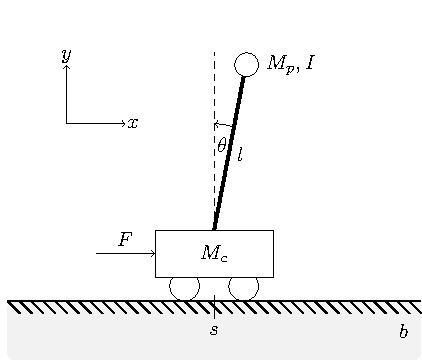
\includegraphics[width=\linewidth]{tikz_inverted_pendulum.pdf}
  \caption{A schematic drawing of the inverted pendulum on a carriage. The mass of the carriage and the pole are given by $M_c$ and $M_p$, respectively. The pole is defined by its length $l$ and its moment of inertia $I$. $b$ is the friction coefficient between the carriage and the floor. The states of the state-space model are the carriage position $s$, its derivative $\dot{s}$, the pole angle with the vertical $\theta$ and its derivative $\dot{\theta}$. $F$ is the applied force. }
  \label{fig:inverted_pendulum}
\end{figure}
The above state space model defines the nominal dynamics $f_{nom}$ of the inverted pendulum. A true disturbance $d_{true}$ is added to the nominal model to form the true dynamics $f_{true}$. Representing a defect in the joint connecting the cart and the pole the disturbance is given by 
\begin{align}
\begin{split}
d_{true} &= 0.1 \theta -0.01 \dot{\theta} + 0.0524\\
&= 0.1 \boldsymbol{z(1)}-0.01 \boldsymbol{z(2)} + 0.0524,
\end{split}
\end{align}
with $\boldsymbol{z}=\boldsymbol{B_z} \boldsymbol{x}$ and 
\begin{equation}
    \boldsymbol{B_z}=
    \begin{bmatrix}
    0 & 0 & 1 & 0\\
    0 & 0 & 0 & 1
    \end{bmatrix}.
\end{equation}
The disturbance only affects $\theta$ which is implemented by setting $\boldsymbol{B_d} = [0, 0, 1, 0]$.
In our example the parameters of the inverted pendulum were set to $M_c=5$, $M_p=2$, $I=0.6$, $l=3$ and $b=0.1$. The implemented MPC has a prediction horizon $N$ of $N=10$ and the number of iterations to optimize the cost function at each time step is limited to ten.
The control formulation aims to stabilize the pole at $\theta=\pi$. Therefore, the cost function $f_c$ is defined to
\begin{equation}
f_c= (\boldsymbol{C_k} \boldsymbol{\mu_x}-\boldsymbol{r(t)})^T \boldsymbol{Q} (\boldsymbol{C_k} \boldsymbol{\mu_x}-\boldsymbol{r(t)}) + R u^2,
\end{equation}
where $\boldsymbol{Q}$ and $R$ are weight matrices/values penalizing the deviation between a selection of mean states $\boldsymbol{C_k}\boldsymbol{\mu_x}$ and the reference signal as well as the amplitude of the input force $F$, respectively. The reference $r$ is defined to $\dot{x}= 0$, $\theta=0$ and $\dot{\theta}=0$.\\
The final cost is defined by
\begin{equation}
f_{end}= (\boldsymbol{C_k} \boldsymbol{\mu_x}-\boldsymbol{r(t)})^T \boldsymbol{Q} (\boldsymbol{C_k} \boldsymbol{\mu_x}-\boldsymbol{r(t)}).
\end{equation}
\subsection{Single-Track System}
The single-track model is a simplified version of the more complex twin-track model, where the front and rear axis only carry one wheel each instead of two.
A schematic drawing of the single-track model including the relevant parameters can be seen in Figure~\ref{fig:singletrack}.
\begin{figure}
  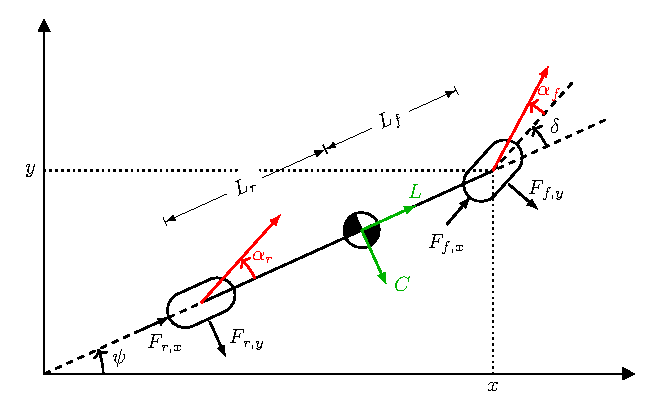
\includegraphics[width=\linewidth]{tikz_singletrack.pdf}
  \caption{A schematic drawing of the single-track model. The vehicle mass and the vehicle moment of inertia (yaw axis) are given by $M$ and $I$, respectively. The distance from the front wheel as well as from the rear wheel to the center of mass are defined by $L_f$ and $L_f$, respectively. $\psi$ is the yaw angle. The forces which act on the rear and front wheel in longitudinal and lateral direction are named $F_{r,x'}$, $F_{r,y'}$, $F_{f,x'}$ and $F_{f,y'}$. The rear-slip angle is $\alpha_r$ and the front-slip angle is $\alpha_f$ }
  \label{fig:singletrack}
\end{figure}

The state-space representation of the single-track model is given by
\begin{align}
\dot{I}_x &= V_{x'} \cos(\psi) - V_{y'} \sin(\psi)\\
\dot{I}_y &= V_{x'} \sin(\psi) + V_{y'} \cos(\psi)\\
\dot{\psi} &= \dot{\psi}\\
\dot{V}_{x'} &=  \frac{1}{M}  (F_{r,x'} + F_{f,x'}*\cos(\delta) - F_{f,y'} \sin(\delta) + V_{y'}\dot{\psi})\\
\dot{V}_{y'} &=  \frac{1}{M}   (F_{r,y'} + F_{f,x'} \sin(\delta) + F_{f,y'} \cos(\delta) - V_{y'} \dot{\psi})\\
\ddot{\psi} &= \frac{1}{I} (F_{f,y'} L_f \cos(\delta) + F_{f,x'} L_f \sin(\delta) - F_{r,y'} L_r)\\
\dot{d_{track}} &= v_{track},
\end{align}
where the steering angle $\delta$, the wheel torque gain $T$ and the track center line velocity $v_{track}$ are inputs. The wheel torque gain is bounded by -1 (maximum deceleration) and 1 (maximum acceleration). Additionally, the steering angle is bounded between -30 degree and 30 degree.
The wheel forces in vehicle coordinates are defined to
\begin{align}
 F_{r,x'} &= \zeta  F_W\\
 F_{r,y'} &= c_r \alpha_r \\
 F_{f,x'} &= (1-\zeta)  F_W\\
 F_{f,y'} &= c_f  \alpha_f, 
\end{align}
where $\zeta=0.5$ is longitudinal wheel torque distribution and $c_f =c_r=14000$ front  and rear cornering stiffness. The is total wheel force $F_W$ given by
\begin{equation}
F_W = T  ( (T>0) 4000+(T<0) 8000 sign(V_{x'}) ),
\end{equation}
where the factor 4000 allows 1g (1 $g M$) acceleration and the factor 8000 2g (2 $g M$) breaking.
The wheel slip angles $\alpha_r$ and $\alpha_f$ are defined by
\begin{align}
\alpha_r &= \text{atan2}(V_{y'}-L_r \dot{\psi},V_{x'})\\
\alpha_f &= \text{atan2}(V_{y'}+L_f \dot{\psi},V_{x'}) - \delta.
\end{align}
 \\
Ideas, theorems, proofs and discussions .....
Ideas, theorems, proofs and discussions .....



%%%%%%%%%%%%%%%%%%%%%%%%%%%%%%%%%%%%%%%%%%%%%%%%%%%%%%%%%%%%%%%%%%%%%%%%%%%%%%%%
\section{EXAMPLES}\label{examples}

Show and discuss simulation examples etc....



%%%%%%%%%%%%%%%%%%%%%%%%%%%%%%%%%%%%%%%%%%%%%%%%%%%%%%%%%%%%%%%%%%%%%%%%%%%%%%%%
\section{CONCLUSIONS}

Summarize the main points (with more details than in the preceding introduction).
The paper should not be between 4 and 8 pages.

%%%%%%%%%%%%%%%%%%%%%%%%%%%%%%%%%%%%%%%%%%%%%%%%%%%%%%%%%%%%%%%%%%%%%%%%%%%%%%%%


\addtolength{\textheight}{-12cm}   % This command serves to balance the column lengths
                                  % on the last page of the document manually. It shortens
                                  % the textheight of the last page by a suitable amount.
                                  % This command does not take effect until the next page
                                  % so it should come on the page before the last. Make
                                  % sure that you do not shorten the textheight too much.

%%%%%%%%%%%%%%%%%%%%%%%%%%%%%%%%%%%%%%%%%%%%%%%%%%%%%%%%%%%%%%%%%%%%%%%%%%%%%%%%


%%%%%%%%%%%%%%%%%%%%%%%%%%%%%%%%%%%%%%%%%%%%%%%%%%%%%%%%%%%%%%%%%%%%%%%%%%%%%%%%
\section*{APPENDIX}

Appendixes should appear before the acknowledgment.

\section*{ACKNOWLEDGMENT}


%%%%%%%%%%%%%%%%%%%%%%%%%%%%%%%%%%%%%%%%%%%%%%%%%%%%%%%%%%%%%%%%%%%%%%%%%%%%%%%%

\bibliographystyle{plain}
\bibliography{mybib}

%\begin{thebibliography}{99}
%\end{thebibliography}

\end{document}
